%% example.tex
%% Jeremy Singer
%% 16 Oct 12

\documentclass{mpaper}

% set bibliography styling
\usepackage{natbib}
\bibpunct{(}{)}{;}{a}{}{;}

\usepackage{pgfgantt}
\usepackage{graphicx}
\usepackage{booktabs}

\begin{document}

\title{Linking QSAR-Based Drug-Target prediction with AlphaFold}
\author{George Iniatis }
\matricnum{2329642i}
\date{April 14, 2023}

\maketitle

\begin{abstract}
Drug-target interactions (DTIs) play a crucial role in drug discovery and pharmacology. However, their experimental determination is time-consuming and limited. Unwanted or unexpected DTIs could cause severe side effects. Therefore, the creation of machine learning models that can quickly and confidently predict whether thousands of drugs and proteins bind together and how much is crucial. 

The project aimed to create a new curated dataset of DTIs and then use this dataset to train machine learning models. Our models were split into two categories, baseline and enhanced, with baseline using just the drug and protein sequence descriptors and the enhanced using our protein structural embeddings derived from AlphaFold's predictions in addition to those descriptors. 

The created embeddings proved to be ineffective. However, our trained models could still prove useful in uncovering interesting relationships that could be investigated further.
\end{abstract}

\hspace{1cm}
\section{Introduction}
\label{sec:Introduction}

Drug-target interactions (DTIs) refer to the interactions of chemical compounds and biological targets, proteins in our case, inside the human body \citep{Sachdev2019}. Given that both proteins and drugs are chemically active molecules in the bloodstream, it would make sense that they interact in some way \citep{DerangedPhysiology}. These interactions usually form an ever-changing, benign and reversible binding where both molecules move through the bloodstream interlocked together \citep{DerangedPhysiology}. The vast majority of drugs administered take this into account and use this process \citep{DerangedPhysiology}. A protein-bound drug is usually too big to pass through a biological membrane like that of a cell. Therefore only the unbound drug, usually in equilibrium with the bound drug, can pass through and produce the desired pharmacological effect, like the treatment of a disease, or the targeting of a tumour \citep{ProteinBindingOverview}. This is done by binding and usually inactivating another protein by inhibiting its function \citep{Lu2020}. This inhibition depends on the specific drug-protein pair and it can take the form of actively blocking the protein's binding sites, altering the protein's structure or preventing the protein from transmitting chemical signals, amongst many others \citep{Mozhaev1982}. Examples include antibiotics and protease inhibitors that have been widely used to combat diseases like Covid-19, Hepatitis C and HIV \citep{Berry2022, Ma2022}.

\hspace{1cm}

Consequently, the degree of how much a drug binds to a protein can enhance or diminish the drug's effectiveness and performance. For example, minimally protein-bound drugs tend to penetrate tissue better and are excreted much faster from the body than those highly bound \citep{Scheife1989}. In contrast, highly protein-bound drugs, usually meaning that the protein binding is so impactful that we have to pay attention to it, tend to last much longer. This is because the protein acts as a drug "depot" that slowly releases the drug into the bloodstream, again keeping the bound and free drug in equilibrium \citep{DerangedPhysiology, ProteinBindingOverview}.

DTIs play a crucial role in drug discovery and pharmacology. However, the experimental determination of these interactions with methods, such as fluorescence assays, is time-consuming and limited due to funding and the difficulty of purifying proteins \citep{Shar2016, Wang2020}. Past quantitative structure-relationship activity (QSAR) studies discussing protein-drug binding focused on testing thousands of drugs with just a single protein that they deemed important enough \citep{Colmenarejo2003, Vallianatou2013}. These studies often did not consider the protein's sequence or structural information, concentrating their efforts on the drug molecules and their descriptors. However, this is not what we aimed to do in this study. Unwanted or unexpected DTIs could cause severe side effects, therefore, the creation of in silico machine learning models with high throughput that can quickly and confidently predict whether thousands of drugs and proteins bind together and how much could be crucial for medicinal chemistry and drug development, acting as a supplement to biological experiments \citep{Shar2016, Wang2020}.

\subsection{Objectives}
\label{subsec:Objectives}

The project aims to gather publicly available data on known drug-target interactions and place them into a new curated dataset. Then, using this new dataset, train multiple machine learning models using QSAR descriptors derived from a drug's chemical properties and a protein's sequence and 3D structural information to predict whether they bind together. Each protein's 3D structure will be extracted from the AlphaFold protein structure database \citep{Jumper2021, Varadi2022} and one of the main challenges of the project will be in creating an embedding, which efficiently encodes the structural information of the protein, that can then be used in our training process. The models' performance should then be evaluated, and a rudimentary system using these models should be constructed.

\hspace{1cm}

\section{Background}
\label{sec:Background}

Given the important nature of the problem, as discussed in Chapter \ref{sec:Introduction}, there have been numerous attempts to construct machine learning models using various methods, techniques, and biochemical properties to predict DTIs.

Classification models try to predict whether a particular drug will bind with a selected protein (Active) or not (Inactive). However, their accuracy will be influenced by the threshold used to separate the two classes as suggested by \cite{Shar2016}, and the definition of a successful binding may vary substantially for different proteins. Regression models can address these problems by trying to predict the drug-binding affinity, which can take multiple forms, with the dissociation constant ($K_d$), the inhibition constant ($K_i$), and the 50\% inhibitory concentration ($IC_{50}$) being the most common amongst them \citep{Jiang2020}. These values are usually represented by their logarithmic versions.

\subsection{Problem Background}

\subsubsection{Proteins Outline}

Proteins are large complex molecules essential to all biological processes in every living thing \citep{AlphaFold_Blog, CellBiologyEssentials}. They help with digestion, blood circulation, and muscle movement, provide structures, and defend our bodies from diseases. They are made from a combination of amino acids, and the interactions between these chains of amino acids make the protein fold. Each amino acids sequence usually maps 1-to-1 to a 3D structure, and that 3D structure defines what the protein does and how it works \citep{LexFridmanVideo}. If a protein is misfolded, it can lead to diseases such as Alzheimer's and Parkinson's \citep{Misfolding_Diseases}. There are about $10^{300}$ ways to fold a protein given its amino acid sequence \citep{Levinthal1969}. An almost impossible-to-solve problem, known as `Levinthal's paradox' or more simply as the `Protein Folding Problem', that nature solves in milliseconds, and a problem that scientists worldwide have been trying to solve for the past 50 years \citep{AlphaFold_Blog, Torrisi2020}. 

\subsubsection{AlphaFold Breakthrough}
\label{subsubsec:AlphaFold}

We are aware of billions of proteins, and the number keeps increasing, but we only know the exact 3D shape of a small minority of these, roughly 170,000 \citep{Jumper2021}. Mapping these proteins using state-of-the-art methods such as X-ray crystallography and nuclear magnetic resonance is costly, time-consuming, and relies on extensive trial and error, making them highly inefficient and unsuitable for high-throughput screening (HTS). So naturally, scientists worldwide wanted to create a system that could predict a protein's 3D structure just by its amino acid makeup. This is precisely what DeepMind tried to achieve by creating an AI system called AlphaFold, trained on the known sequences and structures of the manually mapped-out proteins.

DeepMind's latest AlphaFold AI system, AlphaFold2, provided the first highly accurate and novel computational solution to this problem, not solving it in its entirety but arguably taking a significant step forward \citep{Jumper2021}. This was demonstrated at the 14th Critical Assessment of protein Structure Prediction (CASP), where AlphaFold outperformed all the other entries in the competition and achieved accuracy similar to that of experimental methods. CASP is organised every two years and uses recently discovered protein 3D structures as a blind test for the prediction systems submitted. It serves as the gold-standard assessment for the prediction accuracy of protein structures.

This breakthrough allowed DeepMind to release protein structure predictions covering almost the entire human proteome (98.5\%). This mapping out of previously unknown human protein structures can provide highly beneficial information, allowing science to understand biological processes better and create more targeted, and therefore more effective, interventions \citep{Tunyasuvunakool2021}. 

Discussing AlphaFold in detail is out of the scope of this project. However, it is an incredibly complex state-of-the-art system that directly predicts the 3D coordinates of all heavy atoms for a given protein just by using its amino acid sequence. 

\subsection{Existing Approaches}
\label{subsec:Existing_Approaches}

\subsubsection{Ligand-Based Approaches}

Ligand-based methods are the most widely used and include QSAR and similarity search-based approaches \citep{Acharya2011}. They make use of a drug's chemical and a protein's sequence descriptors without considering the protein's 3D structure \citep{Aparoy2012}. These types of descriptors are discussed in detail in Sections \ref{subsec:Molecular_Descriptors} and \ref{subsec:Protein_Sequence_Descriptors}, respectively.

Such approaches include the classification study conducted by \citet{Wang2020} and the regression study by \cite{Shar2016}. In both studies, machine-learning models were trained, optimised and evaluated to predict drug-target interactions. However, their methodologies varied from one another, using different databases, datasets and tools, clearly expressing the myriad of distinct approaches one can use to solve this problem.

\citet{Shar2016} utilised the \citet{Ki_Database} from the Psychoactive Drug Screening Program (PDSP) \citep{Ki_Database_Paper} to retrieve DTIs. Then for each drug and protein combination used PubChem \citep{PubChem}, ChemSpider \citep{ChemSpider} and DrugBank \citep{DrugBank} to retrieve each drug's structure and UniProt \citep{UniProt_Paper} to retrieve each protein's sequence. Molecular descriptors were then calculated using Dragon \citep{DRAGON} and protein sequence descriptors using PROFEAT \citep{PROFEAT}. These descriptors were then fed into two models, one based on a support vector machine and another based on a random forest. 

\citet{Wang2020} utilised the DTIs datasets of \citet{Yamanishi2008}, split into Enzymes, Ion Channels, GPCRs and Nuclear Receptors. Then for each drug and protein combination used a Position-Specific Scoring Matrix (PSSM), as mentioned in Subsection \ref{subsubsec:PSSM}, to convert the protein sequence into numerical descriptors containing biological evolutionary information and then a discrete cosine transform (DCT) algorithm to extract the hidden features and integrate them with the molecular fingerprints extracted from PubChem \citep{PubChem}, as discussed in Subsection \ref{subsubsec:Molecular_Fingerprints}. These features were then passed to a rotation forest model. 

Both datasets used were relatively small and had less than 10,000 DTI entries, but that did not stop the models trained from achieving excellent predictive performances and even outperforming state-of-the-art models, possibly highlighting the dataset quality and the processes used.

\bigskip

\subsubsection{Receptor-Based Approaches}
\label{subsubsec:Receptor_Based_Approaches}

Receptor-based approaches such as reverse docking try to predict the preferred conformation and binding strength of a compound to a protein pocket \citep{Meng2011}. They are used when the 3D structure of a protein is mapped and large quantities of data are present. However, such methods are only accurate if the 3D structure of a protein is known, but this could be overcome with predicted 3D protein structures.

One such approach was the study conducted by \citet{Jiang2020}, where the structural information of molecules and the predicted structural information of proteins were used, creating two different graphs that were then fed into two graph neural networks (GNN) to obtain their representations. These representations were then concatenated and used to make DTI predictions.

\citet{Jiang2020} utilised the Davis \citep{Davis_Dataset} and KIBA \citep{KIBA_Dataset_1, KIBA_Dataset_2} datasets, with Davis containing selected entries from the kinase protein family, quantified with $K_d$ values, and KIBA containing entries quantified by a combination of kinase inhibitor bioactivities, $K_i$, $K_d$, and $IC_{50}$, called KIBA score.

Graph neural networks have been widely used in various research fields to solve different problems. A graph made of nodes and edges, irrespective of its size, is passed as the input to the GNN, providing a flexible format to extract in-depth information \citep{Jiang2020}. 

The drug graph was constructed using its SMILE notation, which describes its unique chemical structure, taking the atom as nodes and the bonds between them as edges. Then the related adjacency matrix was created. Finally, a selection of node features based on atoms was also used, shown in Table \ref{tbl:Jiang_Atom_Node_Features}.

The protein graph was constructed by predicting the protein's contact map, with a threshold of 8\AA, from its sequence, using a tool called Pconsc4 \citep{Pconsc4}. A contact map is a 2D representation, usually a matrix, of a protein's 3D structure and can be passed directly to a GNN as an adjacency matrix. A formal definition of contact maps can be found in Subsection \ref{subsubsec:Contact_Maps}.

After getting the protein adjacency matrix, the node features were extracted for further processing. Since the graph was constructed with the residues as the nodes, the features should be selected around them. These properties are shown in Table \ref{tbl:Jiang_Residue_Node_Features}, with PSSM being especially important.

Another interesting study, not for DTI prediction, but for protein function prediction, was that of \citet{Gligorijević} where protein sequences and structures were fed into a two-stage architecture model involving a task-agnostic language model and a graph convolutional network (GCN). 

The language model was used to extract residue-level features from PDB sequences, and then these together with contact maps with a threshold of 10\AA, constructed from the protein structures, were fed into the GCN. Their approach, even if it is trying to solve a different problem, uses a very similar procedure to process a protein's 3D structure.

\subsubsection{Contact Maps}
\label{subsubsec:Contact_Maps}

More formally, the contact map of a protein sequence with length L is a `matrix M with L rows and L columns where each element $M_{ij}$ indicates whether the corresponding residue pair, residue i and residue j, are in contact or not', i.e. have a euclidean distance less than a set threshold, usually 6, 8 or 10 \AA.

\begin{table}[!h]
  \centering
  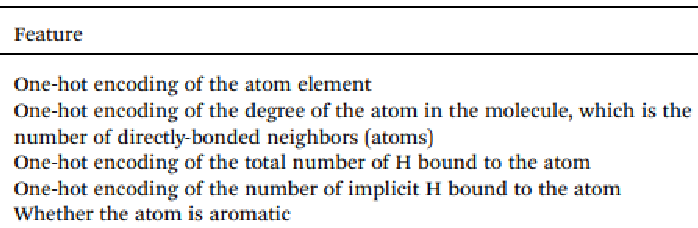
\includegraphics[width=1.0\linewidth]{images/Jiang_Atom_Node_Features.pdf}
  \caption{Part of a table taken from \citet{Jiang2020} showcasing the atom node features used.}
  \label{tbl:Jiang_Atom_Node_Features}
\end{table}

\begin{table}[!h]
  \centering
  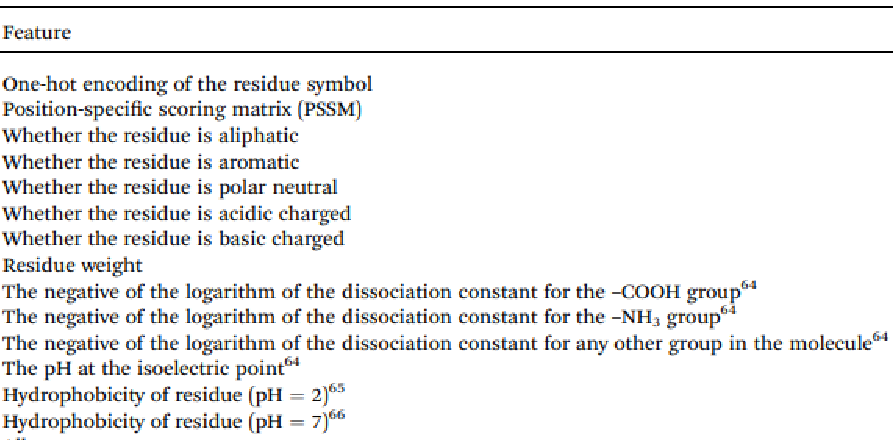
\includegraphics[width=1.0\linewidth]{images/Jiang_Residue_Node_Features.pdf}
   \caption{Part of a table taken from \citet{Jiang2020} showcasing the residue node features used.}
  \label{tbl:Jiang_Residue_Node_Features}
\end{table}

\subsubsection{Valuable Strategies \& Concepts}

All studies highlighted that the complicated structure of proteins and molecules make the creation of accurate representations, the features that will be passed into the models, one of the hardest parts of the whole process. This is an active area of research in it of itself in computer-aided medicine. \citep{Jiang2020}

Both \citet{Jiang2020} and \citet{Gligorijević} agree that the most efficient way to process a protein 3D structure is with a GCN as it generalises convolutional operations on efficient graph-like molecular representations. GCNs have also shown vast success in problems such as the prediction of biochemical activity of drugs and prediction of interfaces between pairs of proteins \citep{Gligorijević}.

\subsubsection{Limitations \& Opportunities}

The studies mentioned in Subsection \ref{subsubsec:Receptor_Based_Approaches} used experimentally obtained protein structures, which as mentioned in Chapter \ref{sec:Introduction} are in short supply and could contain some inherent bias as scientists could be focussing their efforts on specific protein families deemed more important than others, and predicted contact maps from protein sequences in an effort to overcome these limitations. 

The recent advance by AlphaFold, mentioned in Subsection \ref{subsubsec:AlphaFold}, will allow us to use almost the entirety of the proteins in the human proteome not only solving the protein number and bias issues but also arguably providing better quality predicted structural information.

\subsection{Molecular Descriptors}
\label{subsec:Molecular_Descriptors}

Molecular descriptors are numerical features extracted from chemical structures that can be one-dimensional (0D or 1D), 2D, 3D or 4D \citep{Lo2018}.

Although very straightforward to compute or extract, one-dimensional descriptors contain little contextual information on their own. Instead, they describe aggregate information such as counts and chemical properties. In addition, multiple chemical structures can have the same value for a common descriptor, making the usage of just a single 1D descriptor nearly meaningless. Therefore, they are usually expressed as feature vectors of multiple 1D descriptors or used together with descriptors of higher dimensionality.

Two-dimensional descriptors are the most common type found in literature and include molecular profiles, topological indices and 2D auto-correlation descriptors. 

Three-dimensional descriptors extract chemical features and information from 3D coordinate representations and are considered to be the most sensitive to chemical structural differences. However, one of their fundamental limitations is their computational complexity. They include auto-correlation descriptors, quantum-chemical descriptors, substituent constants and surface:volume descriptors. 

Four-dimensional descriptors are an extension of 3D descriptors with the addition that they simultaneously consider multiple structural confrontations. They include descriptors like GRID, Volsurf and Raptor \citep{Lo2018}.

\subsubsection{Molecular Fingerprints}
\label{subsubsec:Molecular_Fingerprints}

The molecular fingerprints of sub-structures can effectively capture the molecular information of drugs by converting them into a bit vector containing 0s and 1s \citep{Wang2020}. Each molecular sub-structure is mapped to a position in the bit vector. If a molecule contains a sub-structure, a value of 1 is assigned to the corresponding bit in the vector or a 0 otherwise \citep{PubChem_Fingerprints}. 

One of the most common molecular fingerprint sources is PubChem \citep{PubChem} which contains 881 molecular sub-structures \citep{PubChem_Fingerprints}, including some padding that needs to be removed before making use of them. 

\subsubsection{Important Molecular Descriptors}

\citet{Shar2016}, after analysing their trained random forest model, found that 2D autocorrelation, topological charge indices and 3D-MoRSE descriptors of compounds were the most essential chemical descriptors in predicting $K_i$. 

\subsection{Protein Sequence Descriptors}
\label{subsec:Protein_Sequence_Descriptors}

Structural and physiochemical descriptors calculated from amino acid sequences are widely used in protein-related machine learning research approaches such as the prediction of structural and functional classes and protein-protein interactions \citep{ProtR_Paper}. The type of descriptors chosen, the numerical representation that encodes the amino acids sequence, is a critical step and can significantly affect the predictive performance of the models a study is trying to train. 

Past web servers and stand-alone programs like PROFEAT \citep{PROFEAT}, which currently is inactive, and PseAAC \citep{PseAAC} that tried to calculate these descriptors were often limited in the number of descriptors they were providing, not flexible enough and difficult to integrate into the machine learning pipeline \citep{ProtR_Paper}.

Protr \citep{ProtR_Paper}, on the other hand, is a comprehensive package, written in R, that generates various numerical representations of proteins and peptides from amino acid sequences, calculating 8 descriptor groups composed of 22 types of commonly used descriptors that include roughly 22,700 descriptor values. In addition, this package also allows users to create custom descriptors, calculate similarity scores between pairs of proteins and provides useful helper functions.

\subsubsection{Position-Specific Scoring Matrix}
\label{subsubsec:PSSM}

Position-Specific Scoring Matrix (PSSM). also known as Position Weight Matrix (PSW), is a typical representation of motifs, which are patterns in biological sequences, and therefore proteins \citep{Jiang2020, Encyclopedia}. Motifs are represented as a vector of values, often probabilities, although different representations can also be found for every possible amino acid or residue at each sequence position. 

\subsubsection{Important Protein Sequence Descriptors}
\label{subsubsec:Important_Protein_Sequence_Descriptors}

\citet{Shar2016}, after analysing their trained random forest model, found that autocorrelation descriptors, amphiphilic pseudo-amino acid composition, and quasi-sequence-order descriptors of protein sequences were found to be the most effective in predicting $K_i$. 

\citet{Ong2007} also evaluated the performance of different standard protein sequence descriptor sets individually and in various combinations and concluded that every set on its own is beneficial. However, the predictive performance of models can be enhanced by utilising different combinations of them. This selection could be made through standard feature selection processes.




\section{Design}
\label{sec:Design}

This chapter will discuss the high-level decisions made to narrow the project's scope.

Although Section \ref{subsec:Objectives} clearly specified our objectives, it did so on a very high level, giving us the freedom to choose the techniques and methods we employed to achieve them. These decisions were primarily influenced by the background research found in Chapter \ref{sec:Background} and could be split into two distinct but interconnected parts that would determine the project's direction.

\subsection{Model Decisions}

The decisions that needed to be made for the creation of our DTI models were the following:

\begin{itemize}
    \itemsep0em 
    \item
    Which machine-learning libraries would we use.
    \item
    What type of models would we train.
    \item
    What models would we train.
    \item
    How would the models be categorised.
    \item
    What metrics and methods would we use to evaluate the models' predictive performance.
    \item
    How would these models be optimised.
    \item
    How would we make the models' predictions more interpretable.
    \item
    What would we use as our dataset labels.
    \item
    How would the dataset be constructed.
    \item
    How would we present our findings.
\end{itemize}

\subsubsection{Machine-Learning Libraries}

We decided to make use of Scikit-Learn \citep{scikit-learn} and Scikit-Optimize \citep{scikit-optimize} as they are well-documented learning libraries with thorough tutorials and examples available.

\subsubsection{Model Types}

To simplify the problem we had first decided to treat it as binary, a drug can bind itself to a protein or not, even though, as mentioned in Section \ref{subsec:Motivation}, the reality is much more complicated and nuanced than that, as anything dealing with the human body. A drug can be highly bound to a particular protein and less so to another, but in the context of this project, we would still consider the drug to bind to both proteins. This was chosen to simplify the problem we would be trying to solve as we felt that trying to predict how much a drug binds to a particular protein would add unnecessary complexity that would be unproductive for the project, especially in the early stages. 

However, after starting to build our dataset we realised that some DTIs had their binding affinity attached in addition to the binary binding relationship and we decided to also build regression models just as a proof of concept which could be the subject of some future work.

\subsubsection{Chosen Models}

The classification models we decided to train were the Dummy Classifier, Logistic Regression, Linear Support Vector Classifier,  K-Nearest Neighbour Classifier, Decision Tree Classifier,  Random Forest Classifier and the Stochastic Gradient Descent Classifier.


The regression model we decided to train were the  Dummy Regressor, Linear Regression, Linear Support Vector Regression, K-Nearest Neighbour Regressor,  Decision Tree Regressor, Random Forest Regressor and Stochastic Gradient Descent Regressor.

\subsubsection{Model Categories}

To tackle the problem we decided to split our models into two distinct categories, baseline and enhanced. The baseline models would serve as one would expect as our baseline, trained on only the selected drug and protein sequence descriptors, and the enhanced models, which would be compared against the baseline ones, trained with the created protein structure embeddings in addition to the selected drug and protein sequence descriptors. 

\subsubsection{Metrics}

To evaluate our models we decided to use numerous metrics for both types of models. This was done not only because it is considered good practice but also to give a more complete view of the models' predictive performance and shortcomings.

The classification models would be evaluated using Accuracy, Precision, Recall, F1 Score and Matthews correlation coefficient (MCC), and the regression models would be evaluated using R2 Score and Negated Mean Absolute Error (MAE), which simply adds a negative sign in front of MAE to make sure that all of our metrics follow the same 'greater is better' principle, making their interpretation easier.

\subsubsection{Model Evaluation}
\label{subsubsec:Model_Evaluation}

To evaluate our models we decided to use holdout test sets and dummy models.

Holdout test sets are subsets of our data that have not been used for either training or validation purposes when training and optimising our model. They are used to estimate a model's real-world performance on previously unseen data.

Dummy models usually predict the most frequent class in the case of classification models and the mean label in the case of regression models, although there are many variations that can be used. These would serve as the random threshold for our models.

\subsubsection{Model Optimisation}
\label{subsubsec:Model_Optimisation}

The model's hyper-parameters would be tuned using the BayesSearchCV function from the Scikit-Optimize \citep{scikit-optimize} library. BayesSearchCV is very similar to the GridSearchCV and RandomizedSearchCV functions offered by Scikit-Learn \citep{scikit-learn}. However, instead of using an exhaustive grid or a random search approach it uses a Bayesian optimisation algorithm which we would argue is much faster than an exhaustive search and much more effective than a random search, particularly when dealing with continuous values. 

Just like the Scikit-Learn functions, BayesSearchCV uses cross-validation to optimise a model for a chosen metric we deem the most important for our specific task. The metrics we chose to optimise our models were the F1 and R2 scores for the classification and regression models, respectively.
 
\subsubsection{Model Interpretability}
\label{subsubsec:Interpretability}

To shine some light into our models' inner workings and to instil some confidence into their predictions, or to at the very least help the user understand what led to a specific prediction, we decided to use \citet{ELI5} to examine the weights of each model's features and \citet{LIME} to explain how these features and their respective values led to a specific prediction.

\subsubsection{Dataset Labels}

For our classification models, the label we would use would be whether a drug or chemical compound can bind with a protein, designated by a 1 and a 0, respectively, and for our regression models, the label would be the logKd value.

\subsubsection{Dataset Sources}

To create our dataset we would make use of the AlphaFold proteins database \citep{Jumper2021, Varadi2022} to extract each protein's structure and sequence and then use PubChem \citep{PubChem} to retrieve the DTIs associated with each protein and the corresponding binding relationship and affinity if available.

Once we had the DTIs we would then retrieve each drug's descriptors, again using PubChem, and each 
protein's sequence descriptors and embeddings, using the ProtR R library \citep{ProtR_Paper}, already mentioned in Section \ref{subsec:Protein_Sequence_Descriptors}, and UniProt database \citep{UniProt_Paper} respectively. Finally, we would retrieve each protein's structural embedding if available. Figure \ref{fig:DTIs_Methodology} nicely summarises our methodology.

\subsubsection{Presenting Findings}
\label{subsubsec:Presenting_Findings}

To present our findings we decided that in addition to the various notebooks we would produce we would also create a very simple \citet{Streamlit} web application to not only showcase the project's work but also to allow people who might not be computer scientists to use our models and make predictions.

\subsection{Embeddings Decisions}

In order to construct our protein structure embeddings we decided to create a neural network that would be trained on a specific classification task, making use of protein 3D structures, involving as many proteins as possible in order to maximise the number of created embeddings. Once the model was trained we would then extract the protein structural embeddings from one of the model layers.

The decisions that needed to be made to create our embeddings were the following:

\hspace{1cm}

\begin{itemize}
    \itemsep0em 
    \item
    What deep-learning libraries would we use.
    \item
    What would be the classification task.
    \item
    How would we use the 3D structures of proteins.
    \item
    How would the dataset be constructed.
    \item
    What would be the model architecture,
    \item
    How would we extract the embeddings,
\end{itemize}

\subsubsection{Deep-Learning Libraries}

We decided to use PyTorch \citep{NEURIPS2019_9015} and PyTorch-Geometric \citep{PyTorch_Geometric} libraries again due to their expanding resources and detailed documentations.

\subsubsection{Classification Task}
\label{subsubsec:Classification_Task}

Given that each protein has one or more molecular functions we decided that it would be the perfect classification task to build our embedding model around. 

The molecular functions of each protein would be extracted from UniProt \citep{UniProt_Paper} and to simplify the problem we decided to only focus on the most prevalent molecular function among our proteins, which was "DNA Binding".

\subsubsection{Protein Structure Representation}
\label{subsubsec:Protein_Structure_Representation}

Inspired by the studies conducted by \citep{Jiang2020, Gligorijević} we decided to use contact maps with a threshold of 10\AA {} to represent the 3D structures of proteins. 

To extract the dense version of the contact maps we decided to use a nanoHUB library \citep{nanoHUB_Library} created precisely for this type of task. We would then convert this dense representation into a sparse one and create our protein graphs which would then be passed into our neural network.

\subsubsection{Dataset Sources}

To create our dataset, as we already mentioned in Subsections \ref{subsubsec:Classification_Task} and \ref{subsubsec:Protein_Structure_Representation}, we would make use of UniProt \citep{UniProt_Paper} and a nanoHUB library \citep{nanoHUB_Library} to retrieve each protein's "DNA Binding" molecular function and contact map, respectively. 

We would also retrieve each protein's amino acid descriptors using the \citet{Peptides} R library, amino acid and protein sequence embeddings again through UniProt and protein sequence descriptors and PSSM using the ProtR R library \citep{ProtR_Paper}. Figure \ref{fig:Embeddings_Methodology} summarises our methodology.

\subsubsection{Model Architecture}
\label{subsubsec:Model_Architecture}

Inspired by the study conducted by \citet{Jiang2020} we decided to use a very similar architecture, showcased in Figure \ref{fig:Embeddings_NN_Architecture}.

Our architecture utilised a protein graph, using a sparse contact map as its adjacency matrix and amino acid descriptors, embeddings and PSSM as its node features, fed into three PyTorch Geometric graph convolutional layers, with ReLU activation and a global mean pooling layer at the end. The protein graph representation would then be flattened using two linear layers and concatenated with the protein sequence descriptors representation which would have passed through three linear layers, again using ReLU activation but also dropout layers. Once concatenated they would be passed through two more linear layers, again with ReLU activation and dropout layers, and a prediction would be made regarding the "DNA Binding" molecular function.

\begin{figure}[!h]
    \centering
    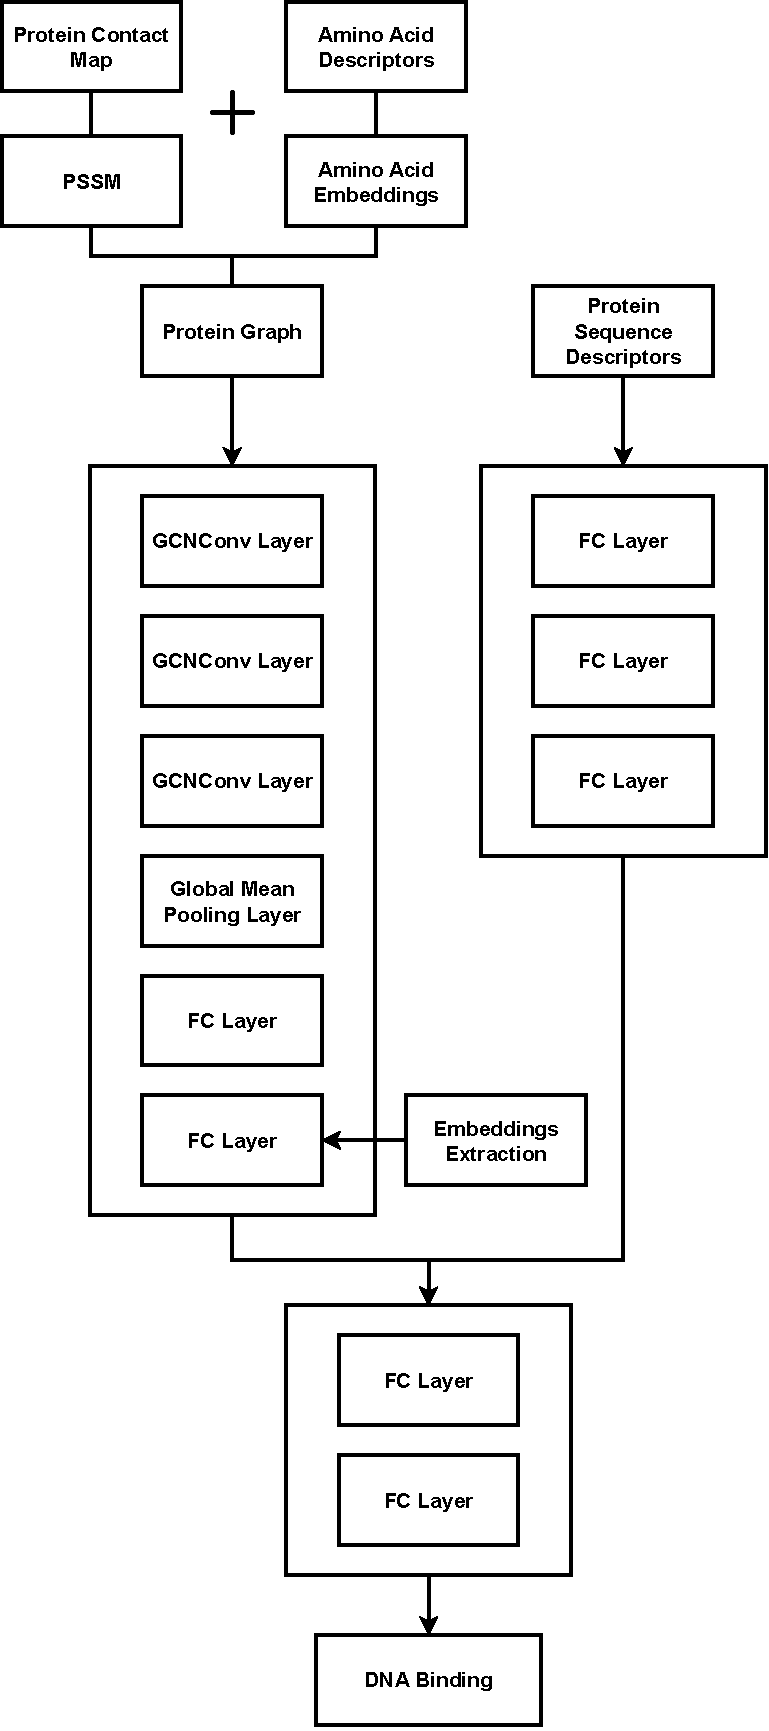
\includegraphics[width=1.0\linewidth]{images/Embeddings_NN_Architecture.pdf}    
    \caption{Figure showcasing our embedding model's architecture.}
    \label{fig:Embeddings_NN_Architecture} 
\end{figure}

\subsubsection{Embedding Extraction}
\label{subsubsec:Embedding_Extraction}

To extract our embeddings from our trained model we would use a forward hook on the second dense linear layer before the concatenation, showcased in Figure \ref{fig:Embeddings_NN_Architecture}, and perform a sequential forward pass over all of our proteins. Each forward pass would extract the embedding and place it into a dictionary which we would then use with our models.

\begin{figure*}[!h]
    \centering
    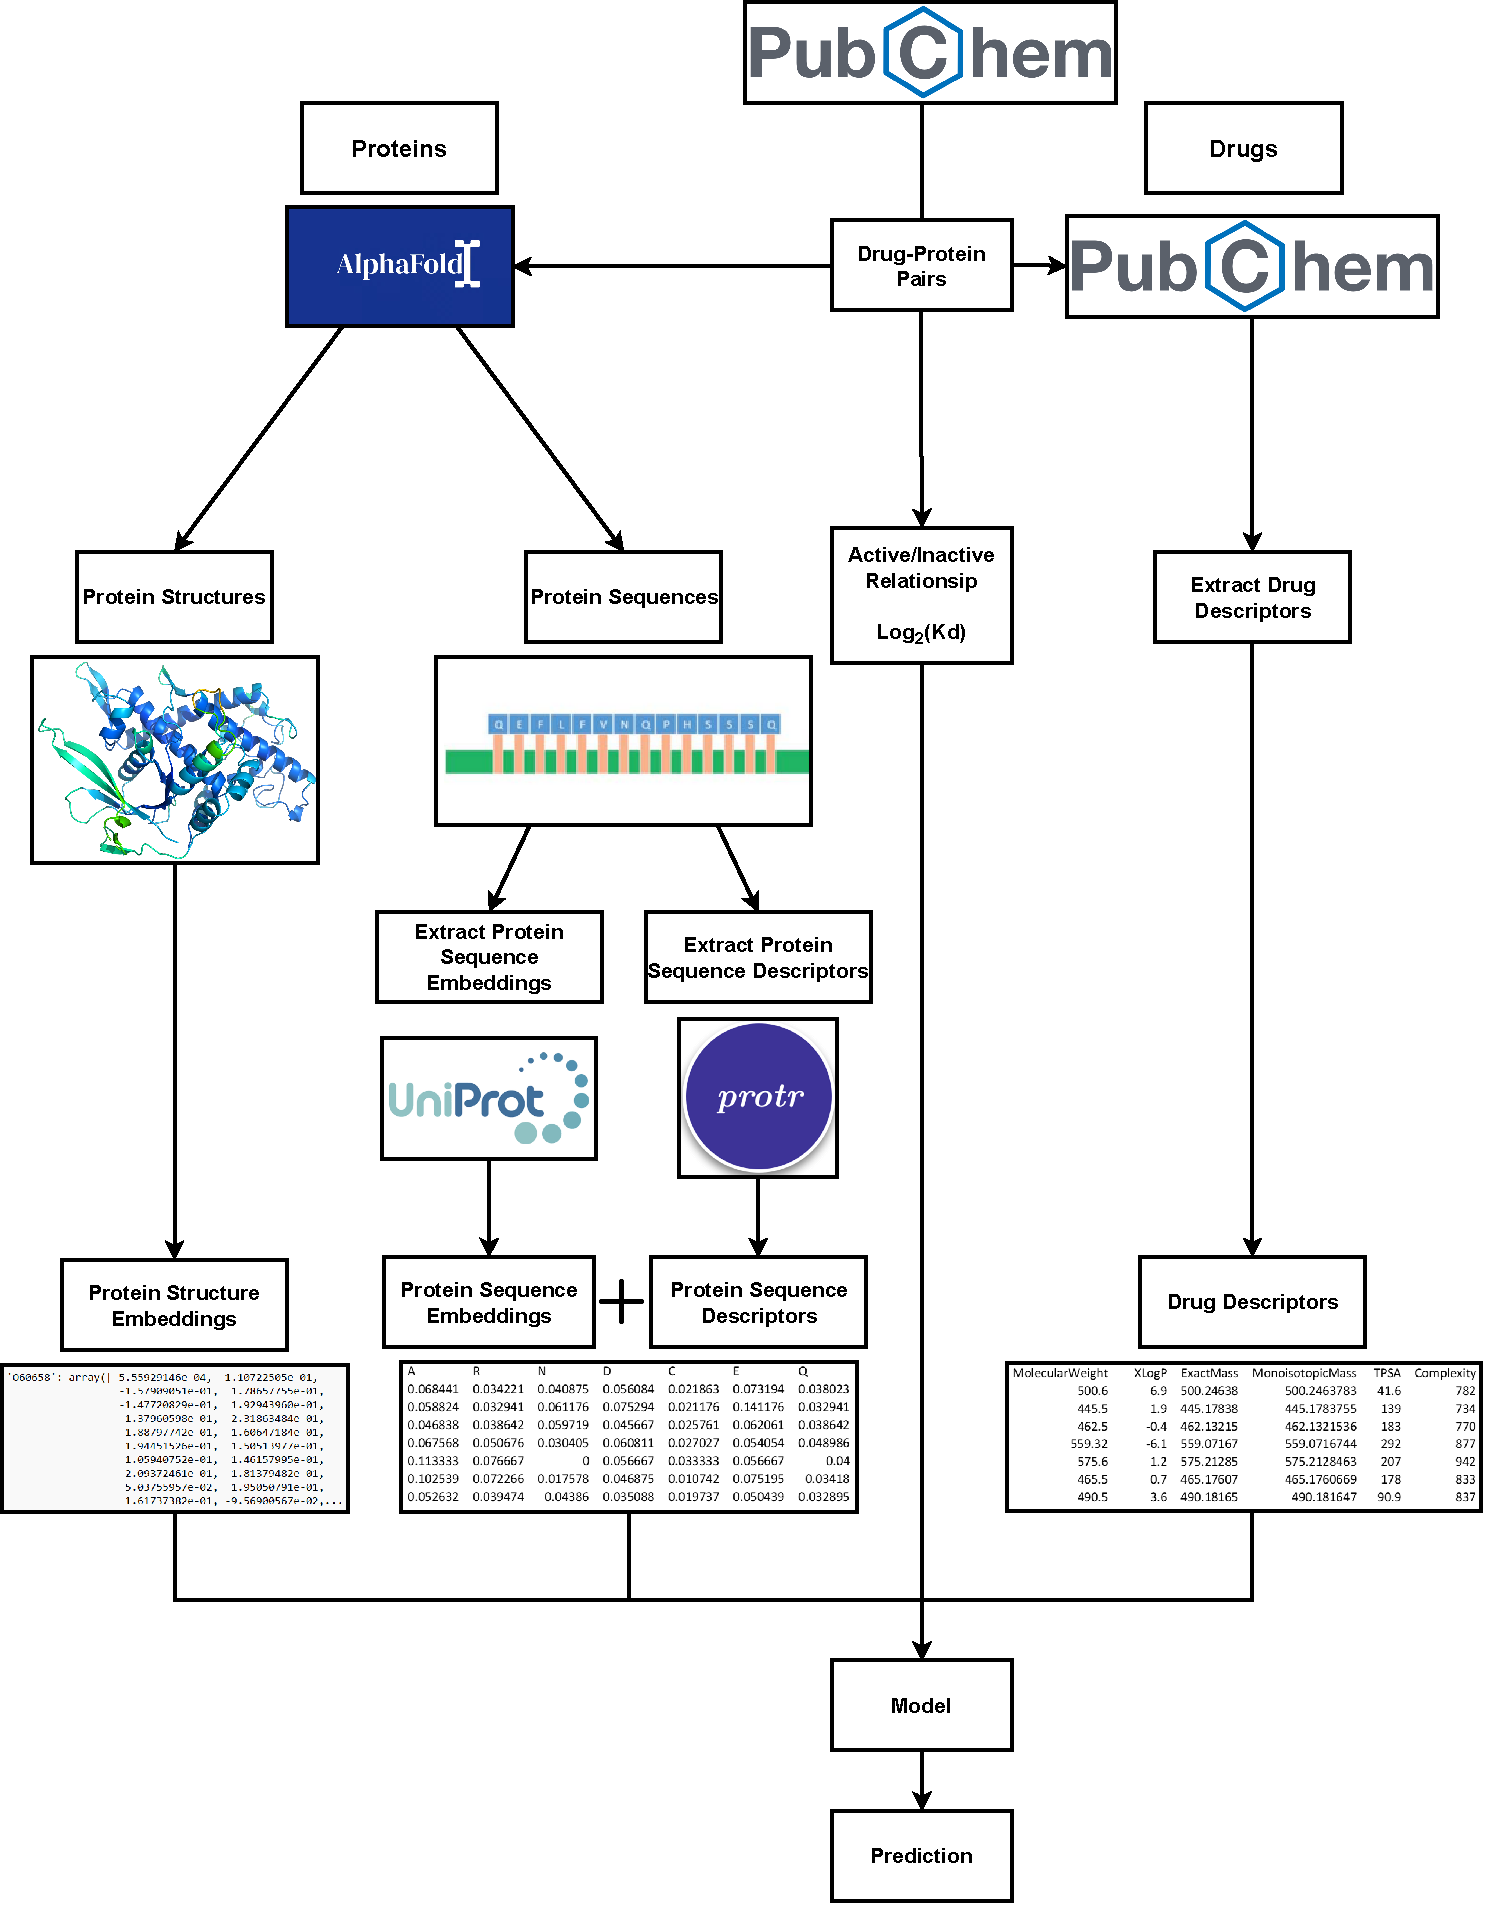
\includegraphics[width=0.95\linewidth]{images/DTIs_Methodology.pdf}    
    \caption{Figure showcasing our methodology behind the DTI models.}
    \label{fig:DTIs_Methodology} 
\end{figure*}

\begin{figure*}[!h]
    \centering
    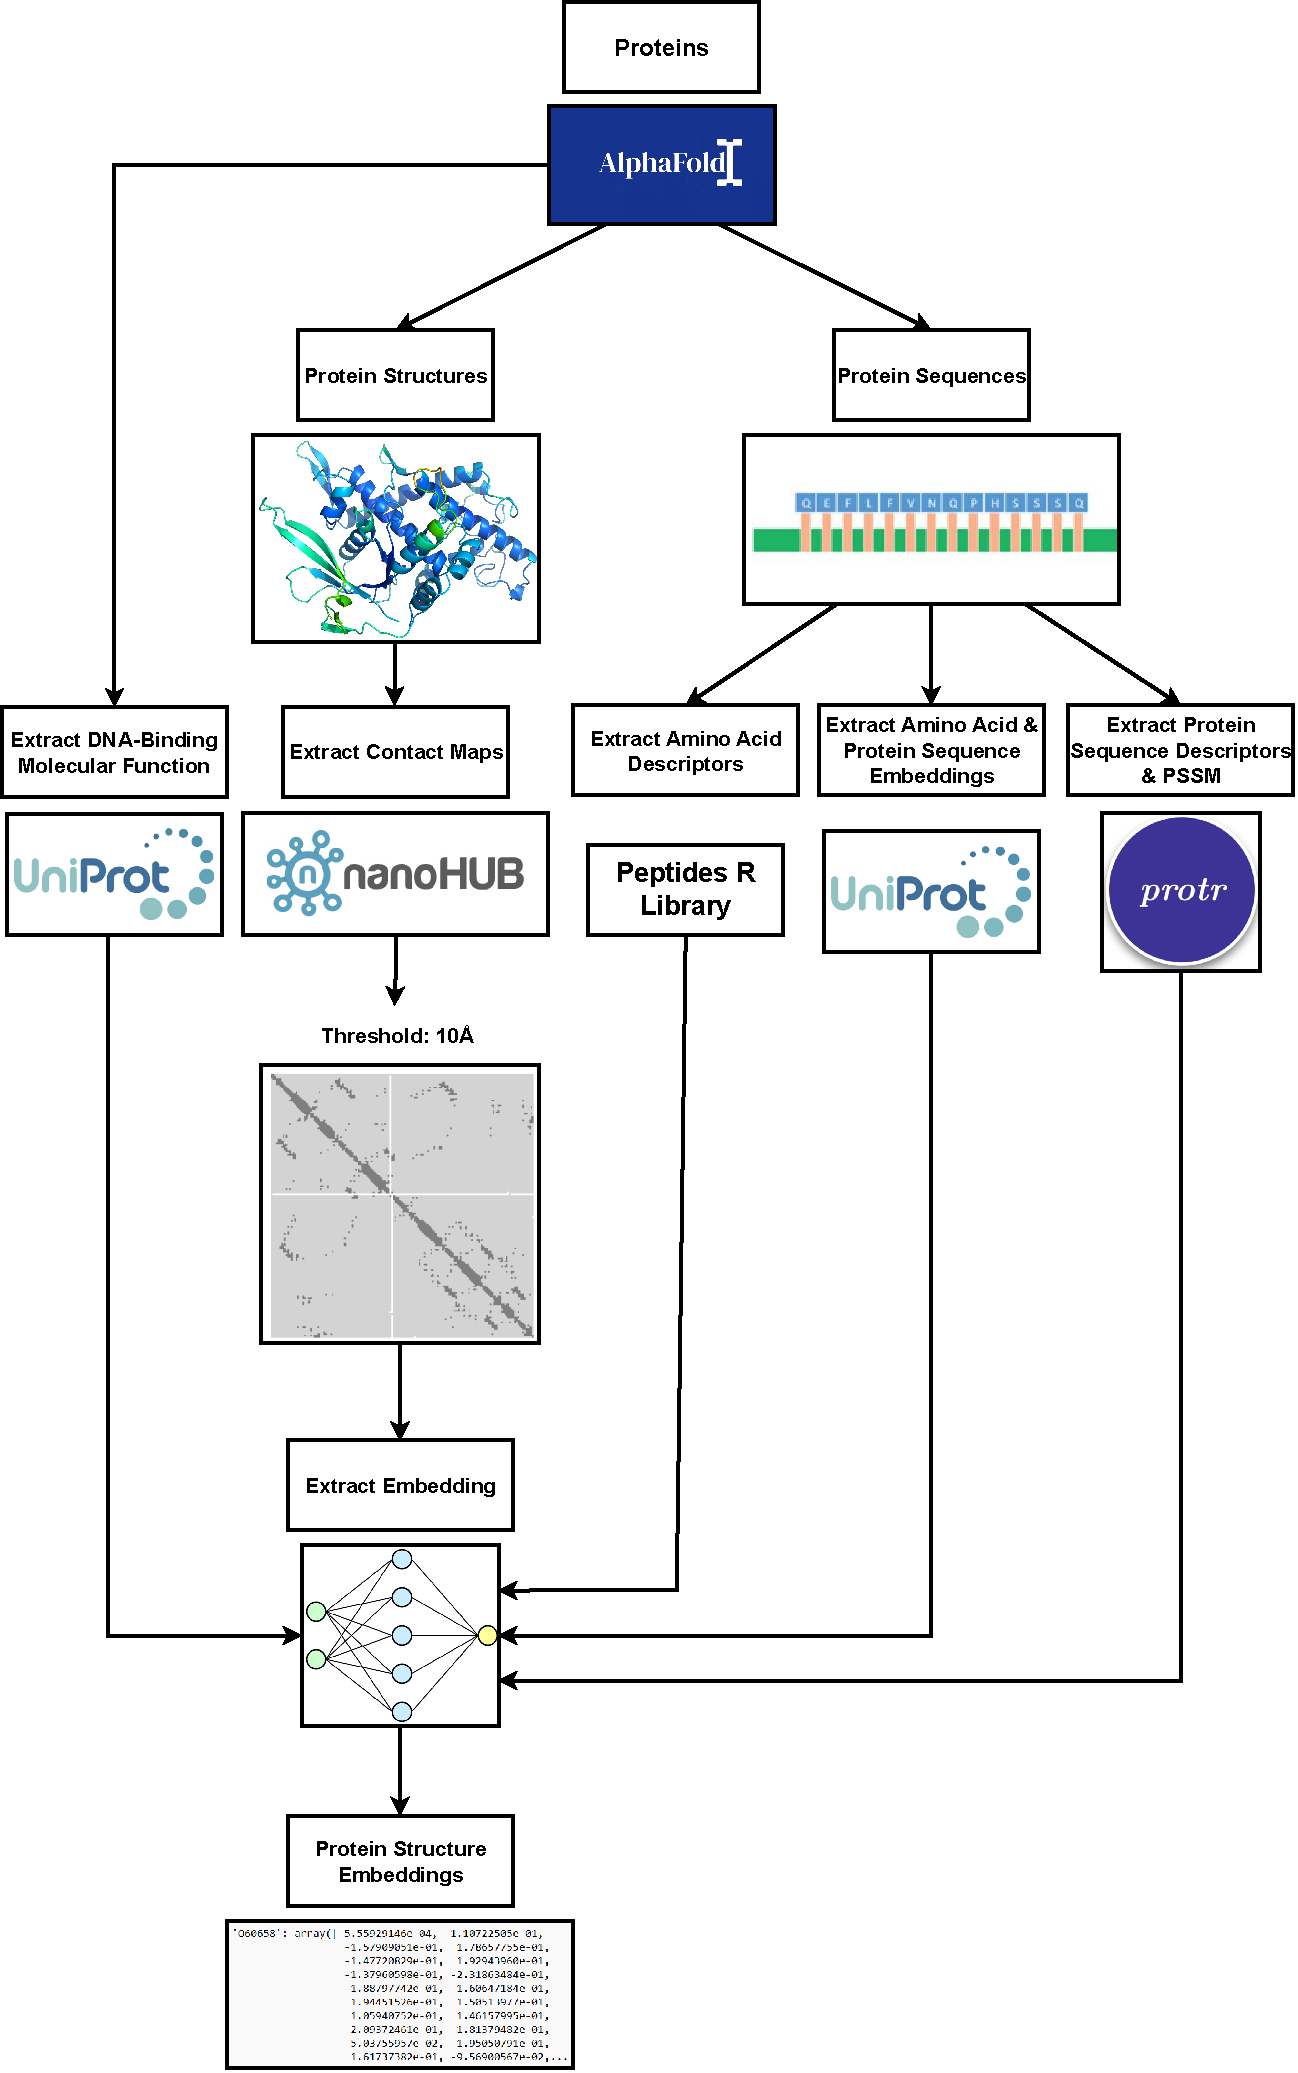
\includegraphics[width=0.78\linewidth]{images/Embeddings_Methodology.pdf}    
    \caption{Figure showcasing our methodology behind the embedding model.}
    \label{fig:Embeddings_Methodology} 
\end{figure*}



\section{Implementation}

This chapter will discuss how our datasets, embeddings and various models were created using the decisions made in Chapter \ref{sec:Design}.

\subsection{Drug-Target Interactions Dataset}

To create our DTIs dataset we started by downloading all the predicted human proteins from the AlphaFold protein structure database \citep{Jumper2021, Varadi2022} and retrieving all the protein accession numbers and sequences. Then using these protein accession numbers \citet{PubChemAPI} calls were made to retrieve the DTIs associated with each protein.

Some proteins had thousands of DTIs available and we felt including every single one would be not only difficult but also counterproductive. Therefore, we decided to place a limit on the number of DTIs retrieved for each protein. This number was arbitrarily set to 100 and if a particular protein's DTIs exceeded that then we would randomly select 100 of them.

Once we had our DTIs it was time to retrieve the descriptors associated with each drug and protein sequence. For each drug we again made use of \citet{PubChemAPI} calls to retrieve every single chemical descriptor stored by PubChem \citep{PubChem}. 

For each protein we used the Protr \citep{ProtR_Paper} library as mentioned in Subsection \ref{subsec:Protein_Sequence_Descriptors} to calculate a large selection of protein sequence descriptors from a variety of descriptors families and UniProt \citep{UniProt_Paper} to extract each protein's sequence embedding. We decided to use a variety of protein sequence descriptor families instead of focusing on a single one because, as we have already discussed in Subsection \ref{subsubsec:Important_Protein_Sequence_Descriptors}, a combination of them can enhance our models' predictive performance.

Once we had everything we needed we performed data cleaning, removing any protein without any DTIs discovered and any dataset entry with missing descriptors, drug or protein related. This process decreased the size of our dataset from 190,028 DTIs to 163,080, with 112,597 classified as having an active relationship and the remaining 50,483 classified as having an inactive one. 

As for the entries having binding affinity available, 72,908 had $IC_{50}$ available, but with just 14 of these being classified as inactive. This was clearly not diverse enough and therefore we moved on to the second most common binding affinity which was $K_d$, with 20,372 entries, 15,007 classified as having an active relationship and 5,365 classified as having an inactive one.

\subsubsection{Feature Selection}
\label{subsubsec:Feature_Selection}

To improve our models' predictive performance, training times but to also discover the drug and protein sequence descriptors holding the most predictive power we decided to use the recursive feature elimination with cross-validation function (RFECV) offered by Scikit-Learn with a random forest classifier or regressor depending on the dataset we would be using and 5-fold cross-validation.

Before running RFECV we decided to reduce the number of tripeptide protein sequence descriptors using principal component analysis (PCA), a dimensionality reduction method, to reduce their size to a number holding 95\% of their variance. As a result, PCA managed to reduce the tripeptide descriptors from 8000 to 2616.

RFECV managed to reduce the features for the classification dataset from 6,474 to 388 and for the regression dataset from 6,474 to 693. 

\subsection{Holdout Test Sets}

As mentioned in Subsection \ref{subsubsec:Model_Evaluation} we decided to use holdout test sets to evaluate our models with previously unseen data. To achieve this we used the train test split function from Scikit-Learn.

Given the nature of our dataset, many proteins can be associated with many drugs, so we could not do the traditional 80/20 split. What we chose to do instead was to take a small subset of our dataset as our test set and remove any proteins and drugs associated with it from the training set. This naturally led to some entries from the dataset not being utilised at all, but we were still left with a substantial amount of training and test data.

For our classification models the training set was 99,705 DTIs and the test set was 816 DTIs and for our regression models the training set was 10,956 DTIs and the test set was 102 DTIs. The same holdout test set will be used for both baseline and enhanced models in order to compare them properly. However, we expect to lose some entries when testing the enhanced models due to not being able to create embeddings for every single protein present in the dataset.

\subsection{DNA-Binding Dataset}

We again started by using all the predicted human proteins from the AlphaFold protein structure database \citep{Jumper2021, Varadi2022} and retrieving all the protein accession numbers and sequences. Then using these protein accession numbers we extracted each protein's molecular functions from UniProt \citep{UniProt_Paper}. As mentioned in Subsection \ref{subsubsec:Classification_Task} we decided to simplify the problem from multi-label to just a single one and that single one was the "DNA Binding" molecular function as it was the most prevalent.

For each protein we used Protr \citep{ProtR_Paper} to retrieve its protein sequence descriptors and PSSM, UniProt \citep{UniProt_Paper} for its protein sequence embedding and amino acids embedding, \citet{Peptides} and more specifically its aaDescriptors function to calculate 66 amino acid descriptors and finally its contact map using a threshold of 10\AA {} using the nanoHUB library \citep{nanoHUB_Library}.

The amino acid descriptors and embeddings, PSSM, and contact maps were all saved as NumPy files in order to easily pass them on to the neural network during its training.

Once we had everything we needed we performed data cleaning, removing any proteins with missing descriptors and any proteins whose acid descriptors and embeddings, PSSM and contact maps were mismatched, meaning having a different amount of amino acids. This process decreased the size of available proteins from 11,202 to 11,034, with 1,989 classified as having a positive "DNA Binding" and 9,045 as having a negative "DNA Binding".

\subsubsection{Feature Selection}

Before running RFECV we again decided to try to reduce the large number of tripeptide protein sequence descriptors using PCA with PCA managing to reduce their number from 8000 to 4813. RFECV was then able to reduce the amount of features from 7757 to 144.

\subsubsection{Training \& Test Sets}

Given that this dataset and the subsequent embedding model were just a means to an end to create as many embeddings as possible we decided against using a holdout test set as the performance of the embedding model was not of interest to us.

\subsection{Embeddings Creation Process}

Following the model architecture discussed in Subsection \ref{subsubsec:Model_Architecture} we trained our neural network using balanced batches of 16 over 50 epochs, which we found were enough for our model to converge. Our model was optimised using Adam with a learning rate of 0.00001 and weight decay of 0.001 and for our loss function we used binary cross entropy loss.

Once the model was trained we used the process discussed in Subsection \ref{subsubsec:Embedding_Extraction} to extract our embeddings, each with 256 dimensions, and place them in a dictionary which we then pickled for easy storage and retrieval.

\subsection{Model Training \& Testing Process}

Our training and testing process was quite simple and used consistently for all models. 

We would first create a pipeline, containing a standard scaler, used to normalise our features by "removing their mean and scaling to unit variance", and our model. The pipeline would then be passed to BayesSearchCV as the estimator along with the model variables we would like to tune, the metric we would like to optimise the model for and the number of folds to use for cross-validation.

All models were optimised using a 5-fold cross-validation except in the case of the dummy and linear regression models as in their case there was nothing to tune and therefore we did not make use of the BayesSearchCV.

Once the models were optimised we evaluated their performance on the respective test set using 95\% confidence intervals of 1000 bootstrapped samples and through the use of confusion matrices in the case of the classification models. 

All models, except the dummy ones, had access to one or both of the model interpretability tools mentioned in Subsection \ref{subsubsec:Interpretability} which in combination with the mentioned evaluation processes and a visualisation of the test set errors could be used to investigate further any of the errors. Our training and test process is summarised in Figure \ref{fig:Model_Training}.

We should also mention that we trained two neural networks, one for classification and one for regression, that used the same architecture as the embedding model, showcased in Figure \ref{subsubsec:Model_Architecture}. Both models were trained using balanced batches of 8 utilising an Adam optimiser with a weight decay of 0.001 and early stopping. 

Their only differences were the learning rates and the loss functions used. The classification neural network used a learning rate of 0.00001 and binary cross entropy loss whereas the regression neural network used a learning rate of 0.000001 and L1 loss.

\begin{figure}[!h]
    \centering
    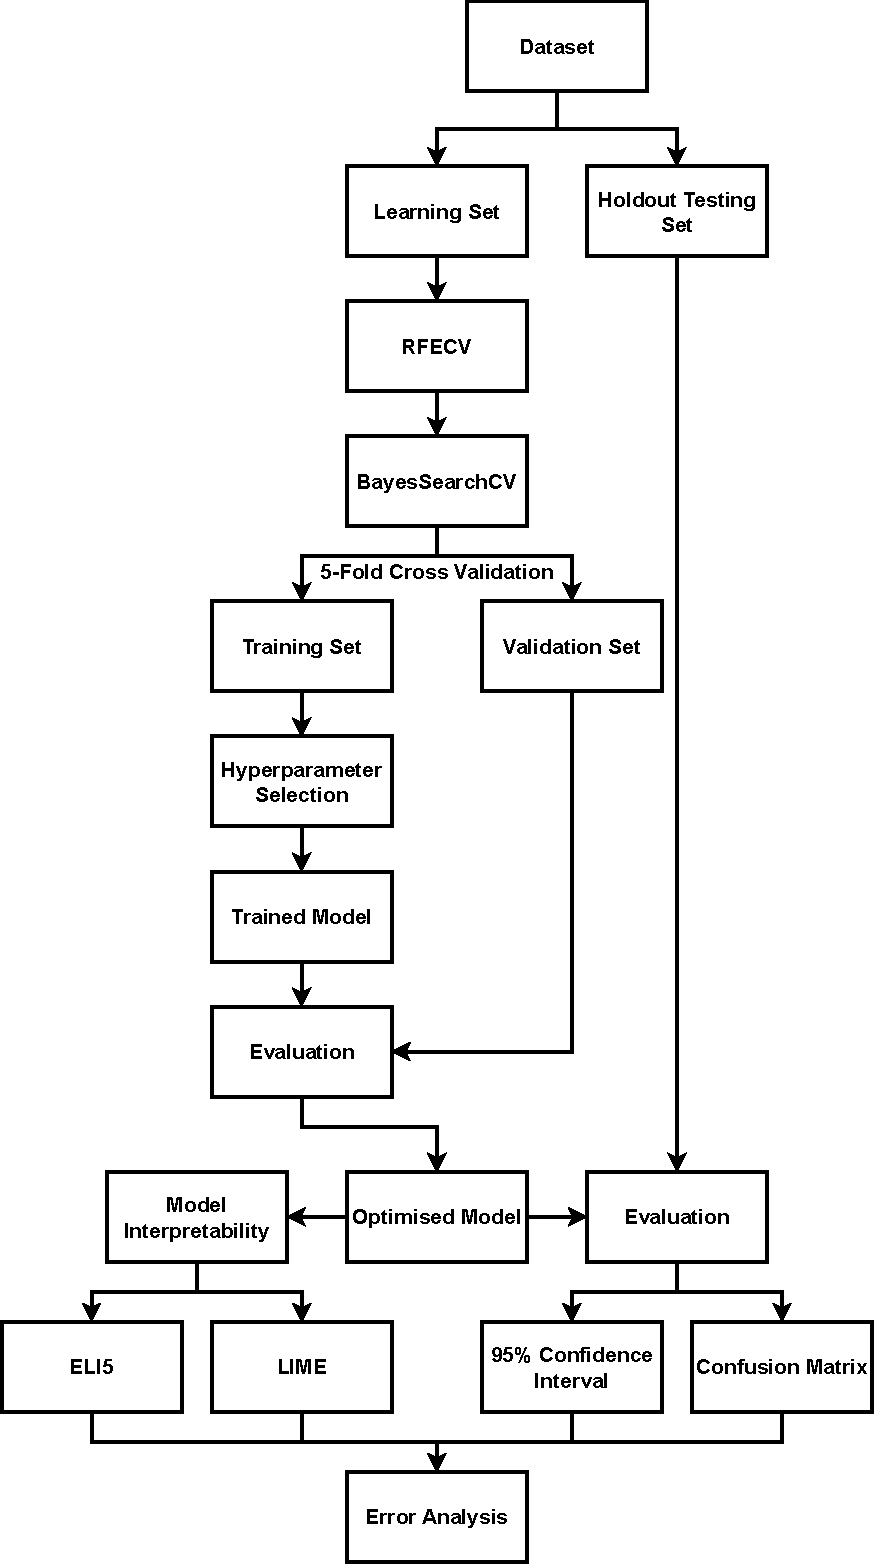
\includegraphics[width=0.85\linewidth]{images/Model_Training.pdf}    
    \caption{Figure showcasing our model training process.}
    \label{fig:Model_Training} 
\end{figure}



% \begin{table}[!h]
% \centering
% \begin{tabular}{lr}
% \toprule
%               Descriptor &  Dimension \\
% \midrule
%          MolecularWeight &       1 \\
%                    XLogP &       1 \\
%                ExactMass &       1 \\
%         MonoisotopicMass &       1 \\
%                     TPSA &       1 \\
%               Complexity &       1 \\
%                   Charge &       1 \\
%          HBondDonorCount &       1 \\
%       HBondAcceptorCount &       1 \\
%       RotatableBondCount &       1 \\
%           HeavyAtomCount &       1 \\
%         IsotopeAtomCount &       1 \\
%          AtomStereoCount &       1 \\
%   DefinedAtomStereoCount &       1 \\
% UndefinedAtomStereoCount &       1 \\
%          BondStereoCount &       1 \\
%   DefinedBondStereoCount &       1 \\
% UndefinedBondStereoCount &       1 \\
%        CovalentUnitCount &       1 \\
%                 Volume3D &       1 \\
%      XStericQuadrupole3D &       1 \\
%      YStericQuadrupole3D &       1 \\
%      ZStericQuadrupole3D &       1 \\
%           FeatureCount3D &       1 \\
%   FeatureAcceptorCount3D &       1 \\
%      FeatureDonorCount3D &       1 \\
%      FeatureAnionCount3D &       1 \\
%     FeatureCationCount3D &       1 \\
%       FeatureRingCount3D &       1 \\
% FeatureHydrophobeCount3D &       1 \\
%     ConformerModelRMSD3D &       1 \\
%    EffectiveRotorCount3D &       1 \\
%         ConformerCount3D &       1 \\
%            Fingerprint2D &     881 \\
% \bottomrule
% \end{tabular}
% \caption{Drug descriptors extracted from PubChem \citep{PubChem}.}
% \label{tbl:PubChem_Descriptors}
% \end{table}

% \begin{table}[!h]
% \centering
% \begin{tabular}{lr}
% \toprule
% Amino Acid Descriptors &  Dimension \\
% \midrule
%     crucianiProperties &       3 \\
%          kideraFactors &      10 \\
%                zScales &       5 \\
%                 FASGAI &       6 \\
%                tScales &       5 \\
%                   VHSE &       8 \\
%                 protFP &       8 \\
%               stScales &       8 \\
%                 BLOSUM &      10 \\
%                 MSWHIM &       3 \\
%                 PSSM   &       - \\
% \bottomrule
% \end{tabular}
% \caption{Amino acid descriptors calculated using the \citet{Peptides} and Protr \citep{ProtR_Paper} R libraries.}
% \label{tbl:Amino_Acid_Descriptors}
% \end{table}

% \begin{table*}
% \centering
% \begin{tabular}{llr}
% \toprule
% Protein Sequence Descriptor Family &      Protein Sequence Descriptor &  Dimension \\
% \midrule
%             Amino acid composition &           Amino acid composition &      20 \\
%                                    &            Dipeptide composition &     400 \\
%                                    &           Tripeptide composition &    8000 \\
%                                    &          Normalized Moreau-Broto &     240 \\
%                    Autocorrelation &                            Moran &     240 \\
%                                    &                            Geary &     240 \\
%                                    &                      Composition &      21 \\
%                                CTD &                       Transition &      21 \\
%                                    &                     Distribution &     105 \\
%                     Conjoint Triad &                   Conjoint Triad &     343 \\
%               Quasi-sequence-order &   Sequence-order-coupling number &      60 \\
%                                    & Quasi-sequence-order descriptors &     100 \\
%      Pseudo-amino acid composition &                           Type I &      50 \\
%                                    &                          Type II &      80 \\
% \bottomrule
% \end{tabular}
% \caption{Protein sequence descriptors calculated using the Protr \citep{ProtR_Paper} R library.}
% \label{tbl:ProtR_Descriptors}
% \end{table*}

\subsection{Streamlit Web App Development}

As mentioned in Subsection \ref{subsubsec:Presenting_Findings} the web app was created to summarise our work and to allow users to perform predictions using our trained models, excluding the neural networks which could not be provided due to size constraints.

We should mention that the model interpretability tools we have already discussed in Subsection \ref{subsubsec:Interpretability} were also made available but not every model can make use of them. \href{https://alphafold-dataset-drug-binding-prediction.streamlit.app/}{\textbf{You can access our web app using this link}}
\section{Results}

\subsection{Models Performance}

We were unable to create embeddings for every single protein in our holdout test sets. Therefore, to get comparable results between the baseline and enhanced models, we had no choice but to remove those entries, marginally decreasing the size of our sets from 816 DTIs for the classification models to 740 and from 102 DTIs for the regression models to 95.

\subsubsection{Classification Models}

Tables \ref{tbl:baseline_classification} and \ref{tbl:enhanced_classification} showcase the predictive performance of our baseline and enhanced classification models and as we can clearly see our embeddings did not have much of an impact, except possibly in the cases of the logistic regression where they seem to have negatively impacted it and the random forest classifier where they seem to have slightly improved performance as we can see from their metrics, and particularly the MCC score.

Our best models in both cases seem to be the K-nearest neighbour and random forest classifier, although all models, except the dummy ones obviously and the decision tree classifier, achieve close enough performances.

\subsubsection{Regression Models}
\label{subsubsec:Regression_Performance}

Tables \ref{tbl:baseline_regression} and \ref{tbl:enhanced_regression} showcase the predictive performance of our baseline and enhanced regression models and it could be argued that our embeddings in this case had a much more evident effect, positive in most cases, except obviously in the case of the linear regression model. However, given that the intervals are so spread out a decisive conclusion cannot be confidently reached.

In the case of the enhanced models, our best models seem to be the K-nearest neighbour regressor and the neural network. As for the case of the baseline models given that all our models achieve a negative R2 score, meaning worse than random, evidenced by achieving worse scores than the dummy regressor, we feel that it would be pointless to point out any of them.

There seem to be some promising results for the regression models and it would be interesting to see what performances they could achieve with a more extensive and diverse dataset than the one we used.

\subsubsection{Model Bias}

All classification models, regardless of type, seem to have particular difficulty in recognising the negative class, meaning an inactive DTI, with actually the number of False Positives surpassing True Negatives in most cases which could be in part explained by the class imbalance present in our dataset. We expect that actively tackling this problem in future work will lead to a noticeable improvement in the predictive performance of the models.

\subsection{Important Descriptors}

As we have previously discussed in Subsection \ref{subsubsec:Feature_Selection}, RFECV was used to find the most important drug and protein sequence descriptors. The intersection between the descriptors found to be important for both classification and regression includes the drug descriptors showcased in Table \ref{tbl:important_drug_descriptors} and the protein sequence descriptors showcased in Table \ref{tbl:important_protein_sequence_descriptors}.

\bigskip
\bigskip

\subsection{Embeddings}

We were able to produce 11,034 protein structural embeddings with 256 dimensions placed into a dictionary which was then pickled for easy storage and retrieval. To visualise them we used PCA to project them into a two-dimensional space and plotted them. 

Looking at Figure \ref{fig:Embeddings_PCA} we can see that most of the embeddings are closely packed together with a few noticeable outliers. However, given the ineffectiveness of our embeddings we cannot draw any conclusions from their spread.

\subsubsection{Performance}

Given that our enhanced machine-learning models, which utilised the embeddings from our transfer learning process, and the neural networks which calculated the protein structural representations optimised specifically for DTI prediction achieved similar performance to that of the baseline models it most certainly appears that we have not efficiently encoded the structural information of proteins.

Considering that we used a very similar deep learning architecture to process the protein contact maps with the successful study conducted by \citet{Jiang2020} we speculate that our choice of 10 \AA {} instead of the 8 \AA {} used by the study mentioned above may have played a significant role in our embeddings ineffectiveness. However, without any further experimentation this remains an unproven theory.

It is also possible that the process used is better suited for predicting the binding affinity of DTIs, given the promising results of Subsection \ref{subsubsec:Regression_Performance}, instead of their binary relationship which may require a more complex representation and processing of protein structures. Such approaches include the studies of \citet{Sofia} and \citet{Lee2022} where they chose a more targeted strategy using each protein's binding pockets instead of its whole structure.

\begin{figure}[!hb]
    \centering
    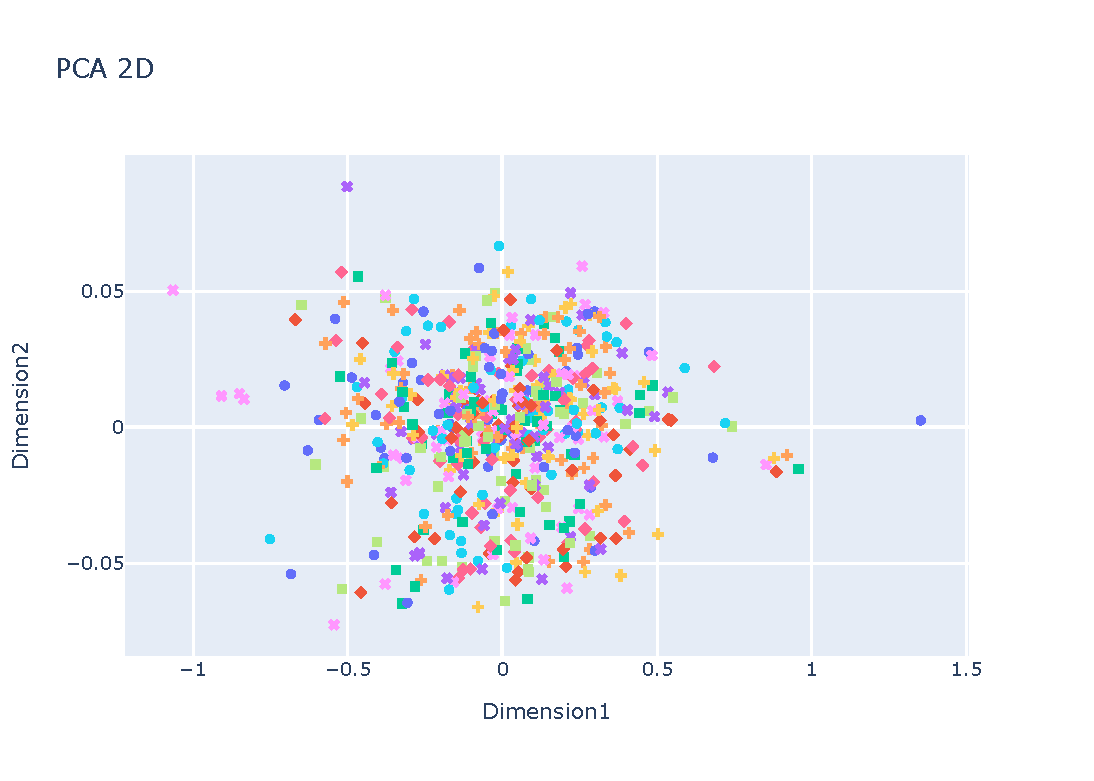
\includegraphics[width=1.0\linewidth]{images/Embeddings_PCA.pdf}    
    \caption{PCA plot of our created protein structural embeddings after projecting them to a two-dimensional space. *Each scatter point is a unique embedding regardless of shape and colour.}
    \label{fig:Embeddings_PCA} 
\end{figure}

\bigskip
\bigskip
\bigskip
\bigskip
\bigskip
\bigskip


\begin{table*}
    \tabcolsep=0.08cm
    \begin{tabular}{llllll}
    \toprule
                                     Model &        Accuracy  &           Recall &        Precision &               F1 & MCC \\
    \midrule
                          Dummy Classifier & 0.68 (0.64-0.72) & 1.00 (1.00-1.00) & 0.68 (0.64-0.72) & 0.81 (0.78-0.84) &                          0 (0-0) \\
                       Logistic Regression & 0.73 (0.69-0.77) & 0.86 (0.83-0.90) & 0.77 (0.73-0.81) & 0.81 (0.78-0.84) &                  0.34(0.24-0.43) \\
      Linear Support Vector Classification & 0.73 (0.69-0.77) & 0.87 (0.84-0.91) & 0.77 (0.72-0.81) & 0.82 (0.78-0.85) &                 0.34 (0.25-0.43) \\
            K-Nearest Neighbour Classifier & 0.75 (0.71-0.79) & 0.83 (0.79-0.87) & 0.81 (0.77-0.85) & 0.82 (0.79-0.85) &                 0.42 (0.33-0.51) \\
                  Decision Tree Classifier & 0.64 (0.60-0.68) & 0.71 (0.66-0.76) & 0.75 (0.70-0.79) & 0.73 (0.69-0.76) &                 0.19 (0.10-0.28) \\
                  Random Forest Classifier & 0.75 (0.71-0.79) & 0.93 (0.90-0.96) & 0.76 (0.72-0.79) & 0.84 (0.81-0.86) &                 0.37 (0.28-0.45) \\
    Stochastic Gradient Descent Classifier & 0.73 (0.69-0.77) & 0.86 (0.83-0.90) & 0.77 (0.73-0.81) & 0.81 (0.78-0.84) &                 0.33 (0.25-0.42) \\
    \bottomrule
    \end{tabular}
    \caption{Testing set (740 DTIs) performance of baseline classification models}
    \label{tbl:baseline_classification}
\end{table*}


\begin{table*}
    \tabcolsep=0.08cm
    \begin{tabular}{llllll}
    \toprule
                                     Model &        Accuracy  &           Recall &        Precision &               F1 &              MCC \\
    \midrule
                          Dummy Classifier & 0.68 (0.64-0.73) & 1.00 (1.00-1.00) & 0.68 (0.64-0.73) & 0.81 (0.78-0.84) &          0 (0-0) \\
                       Logistic Regression & 0.72 (0.68-0.76) & 0.92 (0.89-0.95) & 0.73 (0.69-0.78) & 0.82 (0.79-0.84) & 0.28 (0.18-0.37) \\
      Linear Support Vector Classification & 0.72 (0.68-0.76) & 0.85 (0.81-0.89) & 0.77 (0.73-0.81) & 0.80 (0.77-0.84) & 0.32 (0.22-0.41) \\
            K-Nearest Neighbour Classifier & 0.75 (0.71-0.79) & 0.86 (0.82-0.90) & 0.79 (0.75-0.83) & 0.82 (0.79-0.85) & 0.40 (0.31-0.48) \\
                  Decision Tree Classifier & 0.62 (0.58-0.66) & 0.69 (0.64-0.74) & 0.74 (0.69-0.79) & 0.71 (0.67-0.75) & 0.17 (0.07-0.26) \\
                  Random Forest Classifier & 0.76 (0.72-0.80) & 0.92 (0.89-0.95) & 0.77 (0.73-0.81) & 0.84 (0.81-0.87) & 0.41 (0.32-0.50) \\
    Stochastic Gradient Descent Classifier & 0.73 (0.69-0.77) & 0.92 (0.88-0.94) & 0.75 (0.70-0.79) & 0.82 (0.79-0.85) & 0.31 (0.22-0.40) \\
                            Neural Network &              0.7 &              0.7 &             0.83 &             0.79 &             0.36 \\
    \bottomrule
    \end{tabular}
    \caption{Testing set (740 DTIs) performance of enhanced classification models}
    \label{tbl:enhanced_classification}
\end{table*}

\begin{table*}
    \centering
    \begin{tabular}{lll}
    \toprule
                                    Model & Negated Mean Absolute Error &                     R2 \\
    \midrule
                          Dummy Regressor &      -1.96 (-2.32 to -1.65) &     -0.03 (-0.43 to 0) \\
                        Linear Regression &      -3.57 (-4.39 to -2.78) & -3.10 (-7.20 to -1.28) \\
         Linear Support Vector Regression &      -2.34 (-2.82 to -1.83) & -0.70 (-2.49 to -0.01) \\
            K-Nearest Neighbour Regressor &      -1.50 (-2.06 to -1.02) &  -0.17 (-0.60 to 0.22) \\
                  Decision Tree Regressor &      -3.10 (-3.93 to -2.33) & -2.44 (-7.14 to -0.92) \\
                  Random Forest Regressor &      -2.48 (-2.85 to -2.15) & -0.50 (-1.92 to -0.02) \\
    Stochastic Gradient Descent Regressor &      -2.40 (-3.05 to -1.87) & -0.97 (-2.96 to -0.10) \\
    \bottomrule
    \end{tabular}
    \caption{Testing set (95 DTIs) performance of baseline regression models.}
    \label{tbl:baseline_regression}
\end{table*}

\begin{table*}
    \centering
    \begin{tabular}{lll}
    \toprule
                                    Model &  Negated MAE &                               R2 \\
    \midrule
                          Dummy Regressor &       -1.95 (-2.30 to -1.66) &               -0.03 (-0.29 to 0) \\
                        Linear Regression & -130.78 (-157.40 to -105.42) & -5231.97 (-11775.09 to -2645.58) \\
         Linear Support Vector Regression &       -2.20 (-2.60 to -1.83) &            -0.34 (-1.44 to 0.05) \\
            K-Nearest Neighbour Regressor &       -1.36 (-1.89 to -0.92) &             0.01 (-0.20 to 0.33) \\
                  Decision Tree Regressor &       -2.77 (-3.65 to -1.93) &           -2.35 (-6.89 to -0.61) \\
                  Random Forest Regressor &       -2.43 (-2.82 to -2.10) &               -0.50 (-1.79 to 0) \\
    Stochastic Gradient Descent Regressor &       -1.75 (-2.18 to -1.34) &            -0.09 (-0.65 to 0.15) \\
                           Neural Network &                        -1.56 &                             0.09 \\
    \bottomrule
    \end{tabular}
    \caption{Testing set (95 DTIs) performance of enhanced regression models.}
    \label{tbl:enhanced_regression}
\end{table*}

\begin{table*}
    \centering
    \begin{tabular}{llll}
    \toprule
    MolecularWeight & XLogP & ExactMass & MonoisotopicMass \\
    TPSA & Complexity & HBondDonorCount & HBondAcceptorCount \\
    RotatableBondCount & HeavyAtomCount & AtomStereoCount & DefinedAtomStereoCount \\
    Volume3D & XStericQuadrupole3D & YStericQuadrupole3D & ZStericQuadrupole3D \\ FeatureCount3D &  FeatureAcceptorCount3D & FeatureDonorCount3D & FeatureCationCount3D \\ FeatureRingCount3D & FeatureHydrophobeCount3D & ConformerModelRMSD3D & EffectiveRotorCount3D \\
    ConformerCount3D & Fingerprint2D \\
    \bottomrule
    \end{tabular}
    \caption{Important drug descriptors for both classification and regression.}
    \label{tbl:important_drug_descriptors}
\end{table*}

\begin{table*}
    \centering
    \begin{tabular}{llll}
    \toprule
    CHOC760101.lag4.1 & hydrophobicity.Group3 & secondarystruct.Group1 & prop3.Tr1221 \\
    prop5.Tr1221 & VS562 & Schneider.Xr.N \\
    \bottomrule
    \end{tabular}
    \caption{Important protein sequence descriptors for both classification and regression.}
    \label{tbl:important_protein_sequence_descriptors}
\end{table*}


\section{Conclusion}

This chapter will summarise our work and discuss valuable lessons learned and any potential future work.

\subsection{Summary}

Drug-target interactions (DTIs) refer to the interactions of chemical compounds and biological targets, proteins in our case, inside the human body \citep{Sachdev2019}. They play a crucial role in drug discovery and pharmacology. However, their experimental determination is time-consuming and limited due to funding and the difficulty of purifying proteins \citep{Shar2016, Wang2020}. Moreover, unwanted or unexpected DTIs could cause severe side effects. Therefore, the creation of in-silico machine learning models with high throughput that can quickly and confidently predict whether thousands of drugs and proteins bind together and how much could be crucial for medicinal chemistry and drug development, acting as a supplement to biological experiments \citep{Shar2016, Wang2020}.

The project aimed to gather publicly available data on known DTIs and place them into a new curated dataset. Then, using this new dataset, train multiple machine learning models using simple QSAR descriptors derived from a drug's chemical properties and a protein's sequence and 3D structural information to predict whether they bind together. Our models were split into two categories, baseline and enhanced, with baseline using just the drug and protein sequence descriptors and the enhanced using our protein structural embeddings in addition to those descriptors.

A dataset of 163,080 DTIs was gathered using a variety of databases, libraries and biochemical APIs, subsets of which were used to train both our classification and regression models, evaluated using dummy models, holdout test sets and model interpretability tools. Unfortunately, our embeddings seemed to have little effect on our baseline models, which reasonably falls down to our embeddings creation process.

A Streamlit web app was also created to showcase our work and to allow non-technical users to use our models to make predictions. Model interpretability tools were also made available to allow users to better understand what led to a particular prediction by a model.

Even though our embeddings did not have a significant impact, our high-throughput models could still be used to uncover some interesting relationships between drugs and proteins that could be later confirmed or rejected by molecular docking simulations and actual experimental trials.

\subsection{Reflection}

This project allowed us to work on a fascinating and challenging problem. Even though it could not be called a complete success, we certainly learned a lot, not only about machine learning techniques and best practices but also about bioinformatics in general.

Looking back at the project we should have tried to mitigate the dataset class imbalance, examined further the errors of our models and experimented more with our embedding model's structure and the protein graph we used but also with other extraction methods, possibly utilising each protein's individual pockets instead of its structure as a whole to create the embeddings. However, overall we believe that we have conducted ourselves professionally and responsibly and presented our research in an accurate and unbiased manner. 

\subsection{Future Work}

Multiple project areas could be explored and improved in future work.

The dataset could be improved by expanding it to include more entries with their binding affinity available and trying to reduce the class imbalance through various mitigation techniques. 

A larger improved dataset could lead to improved models, but also different training, optimisation, deep learning architectures, and a thorough investigation with the help of professionals with chemical and biological knowledge into the already created models' errors and blind spots could also be used to create better, more accurate, and robust models.

Finally, the embeddings creation process could also be improved by using a more targeted protein binding-pocket analysis approach instead of the one we used that utilised the protein structure as a whole, which proved ineffective.







{\bf Acknowledgments.}
I want to thank my supervisor Dr. Jake Lever for always guiding me in the right direction and for the wonderful conversations we had over the past two years.

%\setlength{\bibsep}{0pt plus 0.3ex}
\pagebreak
{\footnotesize
\bibliographystyle{agsm}}
\bibliography{msci_paper}
\end{document}
